\documentclass[twoside]{article}

\usepackage[math]{kurier}
\usepackage[sc]{mathpazo}        
\usepackage{graphicx}
\usepackage{subcaption}
\usepackage{algorithm}
\usepackage[noend]{algpseudocode}
\renewcommand{\sfdefault}{kurier}
\usepackage{color,soul}
\usepackage{amsmath}
\usepackage{graphics}
\setlength{\oddsidemargin}{0.25 in}
\setlength{\evensidemargin}{-0.25 in}
\setlength{\topmargin}{-0.6 in}
\setlength{\textwidth}{6.5 in}
\setlength{\textheight}{8.5 in}
\setlength{\headsep}{0.75 in}
\setlength{\parindent}{0 in}
\setlength{\parskip}{0.1 in}

\makeatletter
\def\BState{\State\hskip-\ALG@thistlm}
\makeatother


\newcounter{lecnum}
\renewcommand{\thepage}{\thelecnum-\arabic{page}}
\renewcommand{\thesection}{\thelecnum.\arabic{section}}
\renewcommand{\theequation}{\thelecnum.\arabic{equation}}
\renewcommand{\thefigure}{\thelecnum.\arabic{figure}}
\renewcommand{\thetable}{\thelecnum.\arabic{table}}


\newcommand{\lecture}[4]{
   \pagestyle{myheadings}
   \thispagestyle{plain}
   \newpage
   \setcounter{lecnum}{#1}
   \setcounter{page}{1}
   \noindent
   \begin{center}
   \framebox{
      \vbox{\vspace{2mm}
    \hbox to 6.28in { {\bf \sffamily AA 274: Principles of Robotic Autonomy
                        \hfill Winter 2018} }
       \vspace{4mm}
       \hbox to 6.28in { {\sffamily{\Large \hfill Lecture #1: #2  \hfill}} }
       \vspace{2mm}
       \hbox to 6.28in { {\it \hfill Scribes: #4} }
      \vspace{2mm}}
   }
   \end{center}
   \markboth{Lecture #1: #2}{Lecture #1: #2}

   \vspace*{4mm}
}



%%%%%%%%%%%%%%%%%%%%%%%%%%
%document
\begin{document}
%modify this
\lecture{16}{Sampling-based motion planning}{}{Kaitlin Dennison, Diwaka Ganesan, Jiajie He, Yiwei Zhao}

\section{Introduction} % Kaitlin Dennison
This lecture is on sampling-based motion planning. Please see Chapter 5 of \textit{Planning Algorithms} by Steven Lavelle for more information about these class of algorithms. 

The purpose of sampling-based motion planning is to find an action trajectory $\textbf{u}(t)$ yielding a feasible $\textbf{x}(t) \in X_{free}$ and minimizes \[
J = \int_0^T g(\textbf{x}, \textbf{u}) dt
\] 

This is so say, we want to find a path from start to a goal region that avoids obstacles and possibly optimizes cost such as trading off time with control effort. The reason that motion planning is difficult is that one cannot compute the minimum of $J$ online. We need to develop very fast algorithms that can be computed on-the-fly repeatedly as the robot explores its environment.

One way to do this is to only consider "snap-shots" of the problem within a short horizon: plan a route, move, re-plan, move again, repeat. In this case, the goal region is essential a waypoint along a longer path and we only plan a portion of the route at a time. This reduces the amount of data to compute and allows the environment to change between steps.

\subsection{Configuration Space}
% KAITLIN
The configuration space defines what configurations of the robot are and are not possible. If a configuration is possible, we call it \lq\lq free\rq\rq. The main idea behind motion planning algorithms is to shrink the robots body into a representative point. After we shrink the robot, we must enlarge the obstacles so that we are guaranteed our computed motion plan occurs only within the free areas of the configuration space. The way in which we extend the obstacles is very important. One commonly used technique is to slide the robot's shape around each obstacle by one vertex of the robot. Figure \ref{fig:2Dslide} shows an example of this technique in two dimensions where the gray area is the original obstacle region and the pink area is the enlarged obstacle region - the region where the vertex of the robot cannot enter without a collision occurring. With the enlarged obstacles in the configuration space, a two-dimensional path can be found from start to goal just be considering a two-dimensional point instead of an entire object moving about the space. The set of free poses in the configuration space is denoted $C_{free}$ and the set of poses where an obstacle lies in $C_{obs}$.

\begin{figure}[h!]
  \centering
  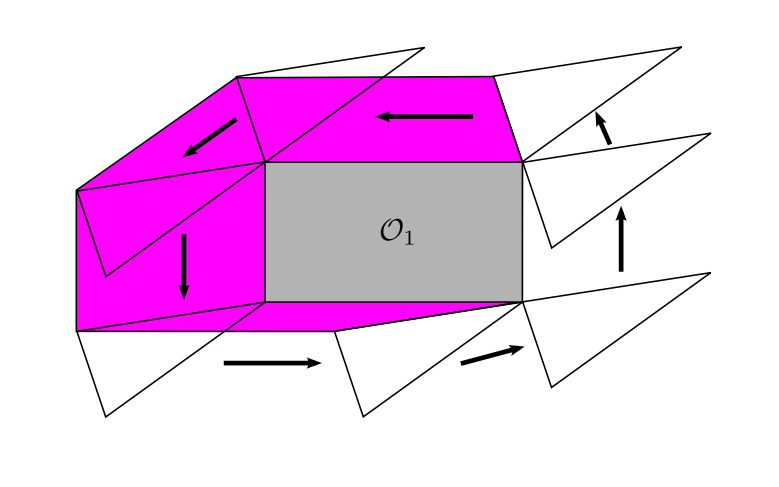
\includegraphics[width=70mm]{SlideRobot.PNG}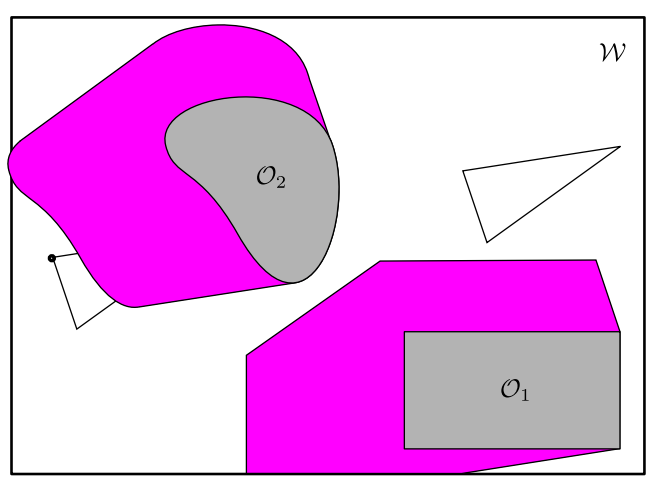
\includegraphics[width=60mm]{SlideRobot2.PNG}
  \caption{(a) Enlarging an obstacle by sliding a triangular-shaped robot around the object by the top-left vertex of the robot. (b) The configuration space with the enlarged obstacles.}
  \label{fig:2Dslide}
\end{figure}

This technique works very well for two-dimensions but starts getting difficult once you add a third and is increasingly harder from there. When considering three dimensions (i.e. heading and two-dimensional position) the configuration space can be built by incrementally fixing the third dimension and enlarging the obstacles in two-dimensions for each increment of the third dimension. This builds layers of the configuration space where each layer is fixed in the third dimension. Figure \ref{fig:3Dslide} shows the steps of building up the configuration space in three-dimensions by incrementally fixing the heading of the robot.

\begin{figure}[h!]
  \centering
  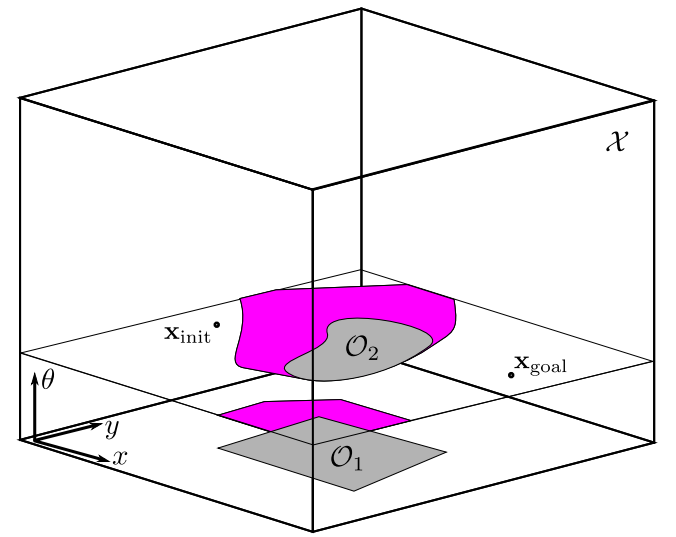
\includegraphics[width=50mm]{3Dslide1.PNG}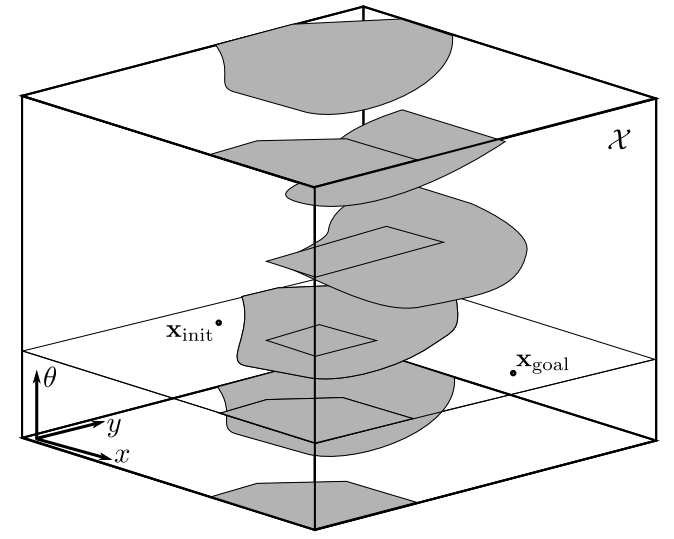
\includegraphics[width=50mm]{3Dslide2.PNG}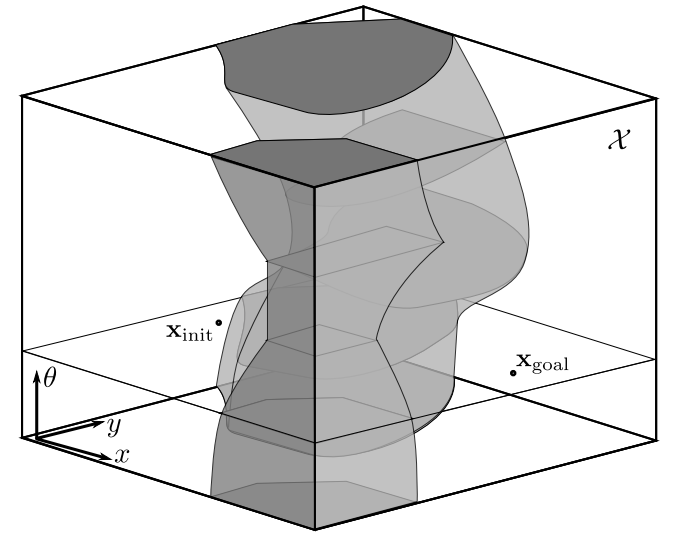
\includegraphics[width=50mm]{3Dslide3.PNG}
  \caption{(a) Fixing $\theta$ and sliding the obstable around in a two-dimensional slice of the configuration space. (b) Stacking multiple fixed slices of the configuration space. (c) Continuous representation of the three-dimensional configuration space.}
  \label{fig:3Dslide}
\end{figure}

\subsection{Approaches to motion planning}

Taking a look at Figure \ref{fig:3Dslide}, it becomes fairly apparent that building a configuration space in three or more dimensions can be extremely cumbersome. Once you include kinematic constraints and other restrictions, it becomes very difficult to compute the positions of the obstacles in the state space. 

There are two approaches to motion planning: \textit{combinatorial planning} and \textit{sampling based planning}. The former computes the entire state space and takes into account all the obstacles in all possible locations in the configuration space. Once we have this complete characterization of $C_{obs}$, we know where $C_{free}$ is, and we can compute a collision-free path. The latter is a randomized algorithm. Random samples, $x_i$, of the state space are generated. If $x_i$ is in $C_{free}$ (black-box probing a collision checker), we keep the sample; if not, we remove it from the sample space. Once all the non-free samples are removed, all of the samples are connected together and then the shortest path is found. This way the entire configuration space does not have to be built and path-finding is only performed on samples that are known to be free.

\section{Overview of sampling-based algorithms} % Dikwaka Ganesan
There are two main categories of sampling-based algorithms for motion planning that we will discuss: geometric, and kinodynamic. 

\subsection{Geometric Algorithms}
In the geometric planning case, the system does not have any dynamics, or the dynamics can be solved using a simple integrator. Essentially, in the geometric case, one can directly control the pose of the robot, not just the first or second derivative of the pose. There are two main algorithms we have to attack geometric planning: Probabilistic Roadmap (PRM) algorithms, and Rapidly-exploring Random Trees (RRT) algorithms. Both algorithms have numerous variations that are used in practice. 

\subsubsection{Probabilistic Roadmaps}
The key insight of a probabilistic roadmap is to avoid the issue of creating a well characterized configuration space (which is computationally expensive), and simply randomly pick samples in the state space to analyze. At a high level, the algorithm proceeds as follows: First, throw a bunch of random samples into your state space (usually a thousand samples will suffice). Then write a collision checker: a computationally cheap algorithm that tests whether the transition between any two samples in the state space results in a collision with an object. Now, the challenge is to connect all the random samples you just generated in some meaningful way. There is a relatively intuitive technique to doing so - simply place an arbitrary disk (called the disk connectivity radius) around each sample $x_i$, and add an edge between $x_i$ and all samples that are within the disk. Before adding the edge, use the collision checker to make sure no collisions happen in those edges. Figure \ref{fig:prm_collision} illustrates this process.

\begin{figure}[h!]
  \centering
  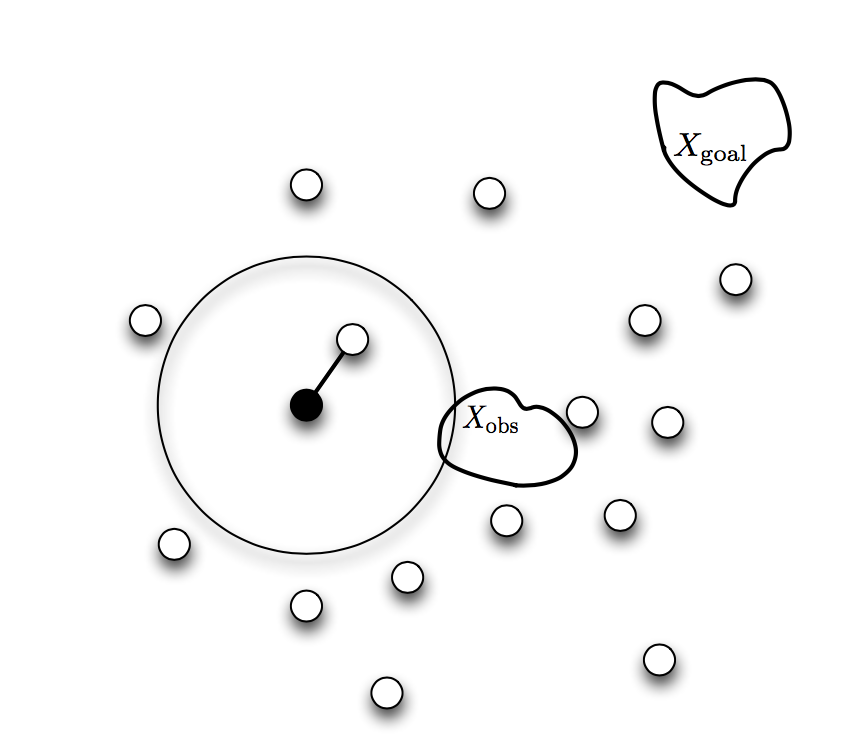
\includegraphics[width=50mm]{prm_collision.png}
  \caption{PRM Collision Checking}
  \label{fig:prm_collision}
\end{figure}


After you iterate through all the samples and add all the relevant edges, you should have a graph that extends from $x_{init}$ to $x_{goal}$. Then, you can use a shortest-path algorithm like $A^*$ to compute the optimal path from the starting pose to the goal pose. 

There is a caveat to PRM in that it tends to provide a good characterization of the state space, but you need to perform many costly collision checks. The PRM algorithm attempts to connect a new node in the state space with all potential neighbors during each collision check, which can add up. 

\subsubsection{Rapidly-exploring Random Trees}
The Rapidly-exploring Random Trees (RRT) algorithm was developed to respond to the issues with Probabilistic Roadmaps. PRMs produce high quality motion plans, but use a very dense characterization of the state space to do so. RRT is a lightweight approach: rather than attempting to characterize the entire state space, we attempt to build a \lq\lq portfolio\rq\rq of trajectories incrementally as the algorithm progresses. Suppose you have already somehow developed two trajectories as seen in Figure \ref{fig:rrt_portfolio}. 

\begin{figure}[h!]
  \centering
  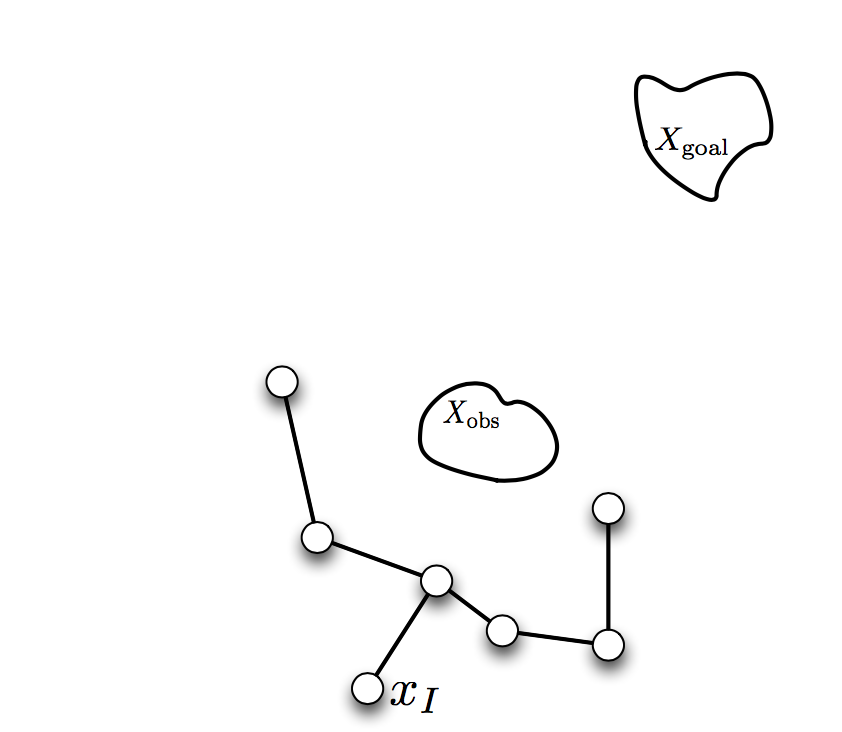
\includegraphics[width=50mm]{rrt_portfolio_of_trajectories.png}
  \caption{Initial \lq\lq portfolio\rq\rq\ of trajectories}
  \label{fig:rrt_portfolio}
\end{figure}

Notice that this portfolio is incomplete - we are trying to expand it to get to our goal region. At each step of the algorithm, we randomly generate a new sample in the state space, Figure \ref{fig:rrt_new_sample}.

\begin{figure}[h!]
  \centering
  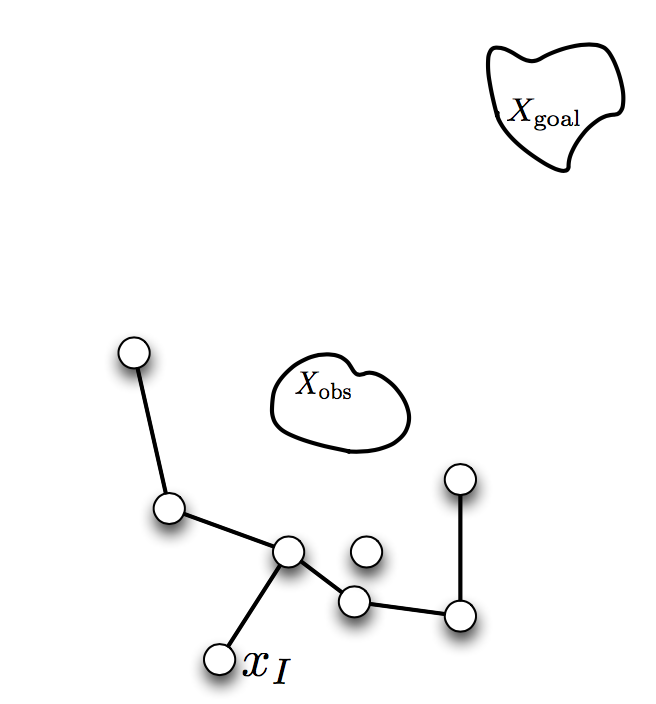
\includegraphics[width=50mm]{rrt_new_sample.png}
  \caption{RRT New Sample}
  \label{fig:rrt_new_sample}
\end{figure}

Then, we must connect this sample somehow to our tree. There are a variety of strategies we can use, but the simplest is to connect the new node to its closest counterpart already on the graph. We keep repeating this process until we reach the goal region. As you may have noticed, the quality of paths that RRT produces can be quite poor. There is an improved method called RRT* that includes an optimization scheme to improve upon RRT.

In RRT*, we can first try to optimize the way we connect a random new node $x_i$ to our graph. After we find the node $x_{near}$ in the graph, we can analyze the neighbors of $x_{near}$ to see if there is a cheaper way to connect $x_i$ to the graph. This method at least introduces a notion of local optimality to the algorithm. We can also check to see if it is possible to get to any of the neighbors of $x_near$ faster if we were to go through $x_i$. Again, remember we must be using the collision checker each time we add an edge to the graph. RRT algorithms find a feasible path very quickly, but these paths can often be sub-optimal. If even one bad step is taken along the way, there is nothing in the RRT algorithm that discourages the exploration of long paths. 

% The following part is done by Yiwei Zhao
\subsection{Fast Marching Tree Algorithm (FMT*)}
Ideally, we want to combine the features of both single-query algorithms (chiefly RRT, which is quick but poor) and multiple-query algorithms (chiefly PRM, which requires a large number of costly collision checks). One way is to run a dynamic programming algorithm called the Fast Marching Tree Algorithm (FMT*) on sample nodes in a way that allow us to grow the tree in cost-to-arrive space. This is generally considered a lazy method, which means it will simply minimize the number of collision checks.

\begin{figure}[h!]
  \centering
  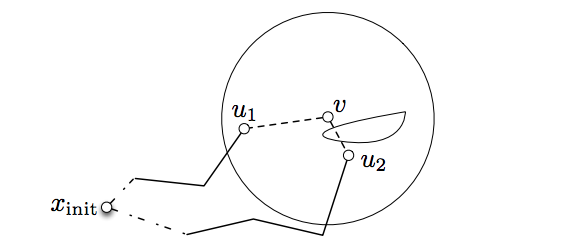
\includegraphics[width=100mm]{fmt.png}
  \caption{Idea of FMT}
  \label{fig:plot_Idea}
\end{figure}

Assuming that we have found a number of trajectories as it shown in Figure \ref{fig:plot_Idea}, we sample a new node, V. In order to connect V to the existing three trajectories we use dynamic programming to look at the optimal cost-to-arrive to each one of the end points of the trajectories. In Figure \ref{fig:plot} these are $u_1$ and $u_2$. We assume this is an incremental algorithm and the proof is done by induction,  so we have already computed the optimal cost-to-arrival to $u_1$ and $u_2$. In order to find the candidate connections we consider the optimal cost-to-arrive for $u_i$ plus the cost of going straight from $u_i$ to V. This process is expressed by equation 16.1:
 
\begin{equation}
    c(v) = \min_{u:\|u - v\| < r_n} \text{Cost}(u, v) + c(v)
\end{equation}

where $u$ are all the node that within radius of the new sample notes and $\text{Cost}(u, v)$ is the cost to connect the note.

In computing, there is a connection we are not accounting for: the presence of the obstacle. After accounting for the obstacle, we rank all the neighbors by their cost and then pick the neighbor that gives us the lowest cost-to-arrive of $v$ and check whether or not there is a collision between the neighbor and the node $v$ by calling collision checker. If so, we choose the second lowest node until we find the lowest neighbor that does not have a collision between it and the node $v$. We will not go through all the nodes in the neighbor and this is the reason that it is lazy dynamic programming. 

For each sample point we usually only perform one collision check because we know we will not keep looking for other members. This is not perfect: sometimes we mistakenly choose the neighbor that has a collision. However, sophisticated analysis shows the number of times that getting the neighbor wrong goes asymptotically to zero as the number of points goes to infinity, which means this algorithm is able to recover an optimal solution even though it only performs one collision check. You can show that the solution quality that you get is very close to PRM with a computational complexity that is very close to RRT thanks to the laziness of FMT*.

The Pseudocode of FMT* can be shown in Figure \ref{fig:plot_Pseudocode}:

\begin{figure}[h!]
  \centering
  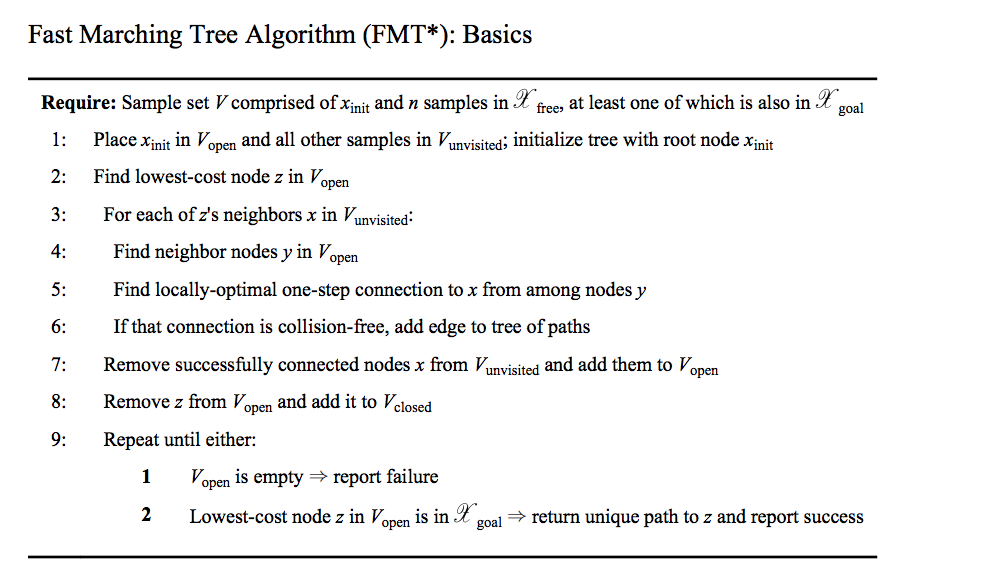
\includegraphics[width=140mm]{Pseudocode.png}
  \caption{Pseudocode for FMT*}
  \label{fig:plot_Pseudocode}
\end{figure}

FMT* is practical because even though the Laziness introduces “suboptimal” connections, such connections are vanishingly rare and FMT* is asymptotically optimal. It's computationally efficient, since the ratio of number of collision-checks for FMT* versus PRM goes to zero. The convergence rate has a bound of order $O(n^{−\frac{1}{d}+\epsilon})$.

% The following part is done by Jeremy(Jiajie) He

\subsection{Deterministic Sampling-Based Motion Planning}
Probabilistic sampling-based algorithms, such as the probabilistic roadmap (PRM) and the rapidly exploring random tree (RRT) algorithms, represent one of the most successful approaches to robotic motion planning, due to their strong theoretical properties (in terms of probabilistic completeness or even asymptotic optimality) and remarkable practical performance. Such algorithms are probabilistic in that they compute a path by connecting independently and identically distributed (i.i.d.) random points in the configuration space. Their randomization aspect, however, makes several tasks challenging, including certification for safety-critical applications and use of offline computation to improve real-time execution. Hence, an important open question is whether similar (or better) theoretical guarantees and practical performance could be obtained by considering deterministic, as opposed to random sampling sequences.

In order to answer this question, we first provide a review of low-dispersion sampling with a focus on $l_2$-dispersion. For a finite set $S$ of points contained in $\chi \in R^d$, $l_2$-dispersion $D(S)$ is defined as:

\begin{equation}
    D(S) := \underset{x\in \chi s \in S}{\text{sup min}} ||s - x||_2
\end{equation}

Intuitively, $l_2$-dispersion quantifies how well a space is covered by a set of points $S$ in terms of the largest Euclidean ball that touches none of the points. The ball radius being smaller would mean that the points are more uniformly distributed. It should be noted that there exist deterministic sequences with $D(S)$ of order $O(n-1/d)$ ($d$ denotes the number of dimensions), referred to as low-dispersion sequences. However, such a sequence minimizing $l_2$-dispersion is only known for $d = 2$.\\

One deterministic sampling-based motion planning algorithm is gPRM (for generic PRM). 

\begin{algorithm}
\caption{gPRM}\label{euclid}
\begin{algorithmic}[1]
\State $\textit{V} \gets \{x_{init}\} \cup \textit{SampleFree(n)}; E \gets \emptyset$
\For {\text{all} $v \in V$} 
\State $X_{near} \gets  \textit{Near(V$\backslash$\{v\},v,$r_{n}$)}$
 \For {$x \in X_{near}$} 
  \If {\textit{CollisionFree(v,x)}}
  	\State $E \gets E \cup \{(v,x)\} \cup \{(x,v)\}$
  \EndIf
  \State \textbf{end if}
 \EndFor
 \State \textbf{end for}
\EndFor
\State \textbf{end for}
\State \textbf{return} $\textit{ShortestPath($x_{init},V,E$)}$
\end{algorithmic}
\end{algorithm}

To discuss the optimality of gPRM, let $c_n$ denote the arc length of the path returned by gPRM with n samples. If
\begin{enumerate}
\item sample set $S$ has dispersion $D(S)<=\gamma n^{-1/d}$ for some $\gamma > 0$
\item $n^{1/d} r_n \rightarrow \infty$
\end{enumerate}
then $\lim_{n \to \infty} c_n = c^*$, where $c^*$ is the cost of an optimal path.

As a derandomized version of PRM, gPRM can achieve asymptotic optimality with a smaller connection radius ($r_n \in \Omega((1/n)^\frac{1}{d})$) than random sampling ($r_n \in \Omega((\log(n)/n)^\frac{1}{d})$) so it requires less computation. Besides, it also has computational and space complexity of $O(n)$ as lower bound, compared with $O(nlog(n))$ for random sampling. Moreover, it has deterministic convergence rate:

\begin{equation}
    c_n <= \left(1+\frac{2D(S)}{r_n-2D(S)}\right)c ^{(\delta)}
\end{equation}

where $c ^{(\delta)}$ is cost of shortest path with strong $\delta$-clearance and assume that $r_n > 2D(S)$. This deterministic convergence rate is instrumental to certification of sampling-based planners. Thus, deterministic sequences appear to provide superior performance.


\section{Kinodynamic Planning}
The  basic  geometric case,  where  a  robot  does  not  have  any constraints on its motion and only an obstacle-free solution is required, is well-understood and solved for a large number of practical scenarios. On the other hand, robots do usually have stringent  kinematic/dynamical constraints on their motion, which in most settings need to be properly taken into account.

\textit{Kinodynamic motion planning} problems are those where feasible paths are subject to differential constraints in addition to obstacle avoidance. There are two versions of kinodynamic planning problems: driftless case and drift case. \textit{Driftless control-affine systems} are those with well understood conditions for small time local controllability and established methods for local steering. Trajectories x in the configuration space must satisfy $\dot{x} = \sum_{i=1}^{m}g_i(x)u_u$. \textit{Control-affine systems} with drift are difficult in general to guarantee local controllability and local steering is known only for special cases. The dynamics can be described as $\dot{x} = Ax + Bu + c$.

Figure \ref{fig:kino} shows the trajectories planned by DFMT* for Reeds-Shepp car (driftless case) and double integrator system (drift case). Note how the trajectories differ between the two systems.

\begin{figure}[h!]
    \centering
    \begin{subfigure}[b]{0.4\linewidth}
      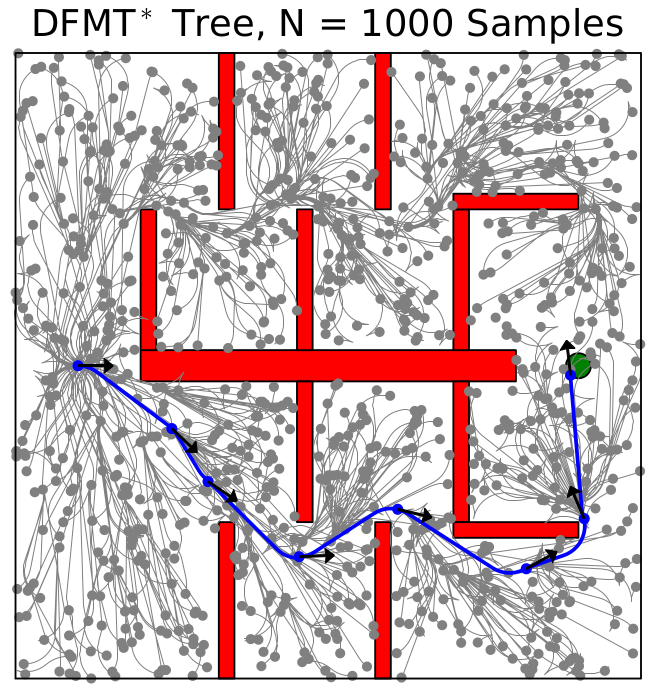
\includegraphics[width=\linewidth]{driftless.png}
      \caption{Reeds-Shepp car}
    \end{subfigure}
    \begin{subfigure}[b]{0.4\linewidth}
      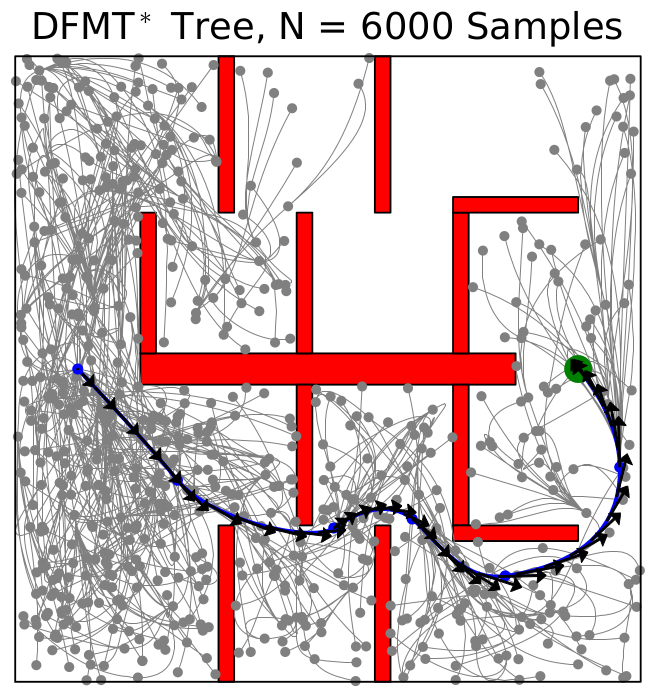
\includegraphics[width=\linewidth]{drift.png}
      \caption{Double integrator system}
    \end{subfigure}
    \caption{DFMT* Tree in driftless case (left) and drift case (right)}
    \label{fig:kino}
  \end{figure}

\end{document}